\subsection{常见NLP任务}

\subsubsection{命名实体识别}
NLP中的命名实体识别(Named Entity Recognition)指的是将识别出文本中描述实体的词汇, 比如人名、地名、组织机构名、股票基金、医学术语等, 更一般地讲, 不同的领域会有不同的实体, 用于描述该领域内的实体对象. NER的目的就是识别出文本中实体与其他文本的边界和实体的类别. 主要以下几个难点: 
\begin{itemize}
	\item 实体的数量是无穷的. 不同的领域会有不同的实体, 且实体并不是定量的, 会不断的增加
	\item 实体的构词灵活. 同一个实体可能会有多个名字, 比如实体的简写;实体也可能是嵌套形成的
	\item 类别模糊. 同一个实体在不同的语境下可能会有不同的类别
\end{itemize}

命名实体的识别, 从某个角度来看可以视作一个序列标注问题. 具体做法是将命名实体附着到{B, M, E, S}标签. 其实, 词性标注问题也可以以这样的方法来处理. 更一般地看, 词性标注与命名实体识别是同一个问题, 它们都需要对文本进行分词, 词性标注中的词性和NER中的实体类别是等价地. 

\subsubsection{语法分析}
分析句子中的语法结构并将其表示为容易理解的结构(通常为树形结构). 
\paragraph{短语结构树}根据上下文无关文法将句子/短语分解为树状结构. 短语结构语法(上下文无关文法)描述了如何自定向下地生成一个句子, 同样句子/短语也可以通过短语结构语法进行分解. 这其实和编译原理中的上下文无关文法是很类似的, 也是通过很多产生式进行推导, 那么是否可以使用编译原理中的词法分析来解决这个问题呢?

\paragraph{依存句法树}关注的是句子中词语之间的语法关联系, 并将其约束为树形结构. 在句子中, 如果一个词语修饰另一个词语, 则称修饰词为从属词, 被修饰词为支配词, 两者之间的语法关系称为依存关系, 在可视化时, 由支配词指向从属词. 依存句法树描述了句子中的各个词之间的依赖关系, 一般约定同一个词不能依存于多个词. 

\textbf{复合性原理}: 一个复杂表达式的意义是由其各组成部分的意义以及结合它们的规则决定的. 通过将句子分解为短语、分解短语为单词, 下游应用会得到更多更深层次的结构化信息. 

\subsubsection{序列标注}
通常也可以看作是token级别的分类问题: 对每一个token进行分类. token级别的分类任务通常指的是为为文本中的每一个token预测一个标签结果, 如命名实体识、词性标注等. 
\begin{itemize}
	\item NER (Named-entity recognition 名词-实体识别) 分辨出文本中的名词和实体 (person人名, organization组织机构名, location地点名...).
	\item POS (Part-of-speech tagging词性标注) 根据语法对token进行词性标注 (noun名词, verb动词, adjective形容词...)
	\item Chunk (Chunking短语组块) 将同一个短语的tokens组块放在一起. 
\end{itemize}

\subsubsection{问答系统}
问答式信息检索是一种允许用户以自然语言方式询问, 系统从单语或多语文档集中查找并返回确切答案或者蕴含答案文本片断的新型信息检索的方式. 问答系统分类如Fig.\ref{fig:qa}所示. 
\begin{figure}[h]
	\centering
	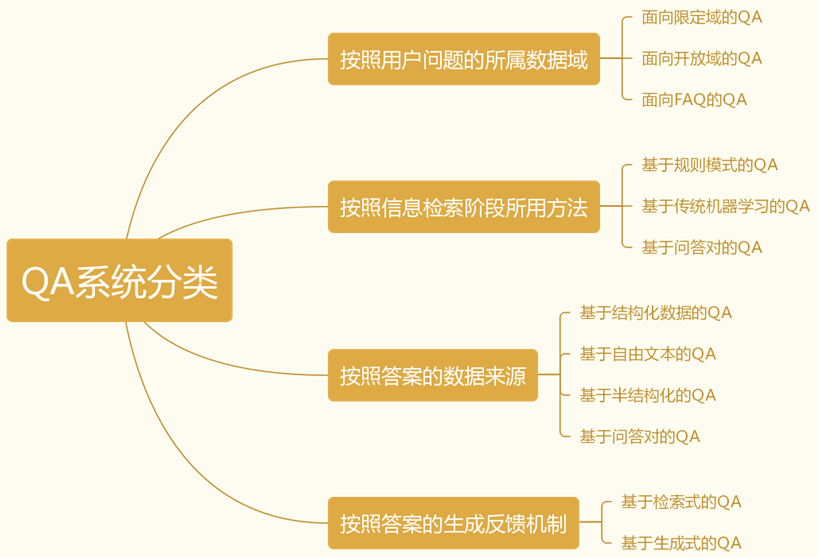
\includegraphics[width=.7\textwidth]{pics/qa.png}
	\caption{问答系统分类, 源图\href{https://blog.csdn.net/sinat_33231573/article/details/83473741}{出处}}
	\label{fig:qa}
\end{figure}









\subsection{预训练}
预训练在很多领域上都有应用, 如CV、NLP. 当用深度学习来解决一个任务时, 使用的深度模型通常会包含很多参数, 我们需要使用大量的数据来更新我们的参数使之能够在特定的任务上取得不错的效果. 一般, 我们会对模型的参数初始化, 然后使用大量带标签的数据来更新模型参数. 

但实际情况是, 带标签的数据总是很少的. 

\begin{figure}[h]
	\centering
	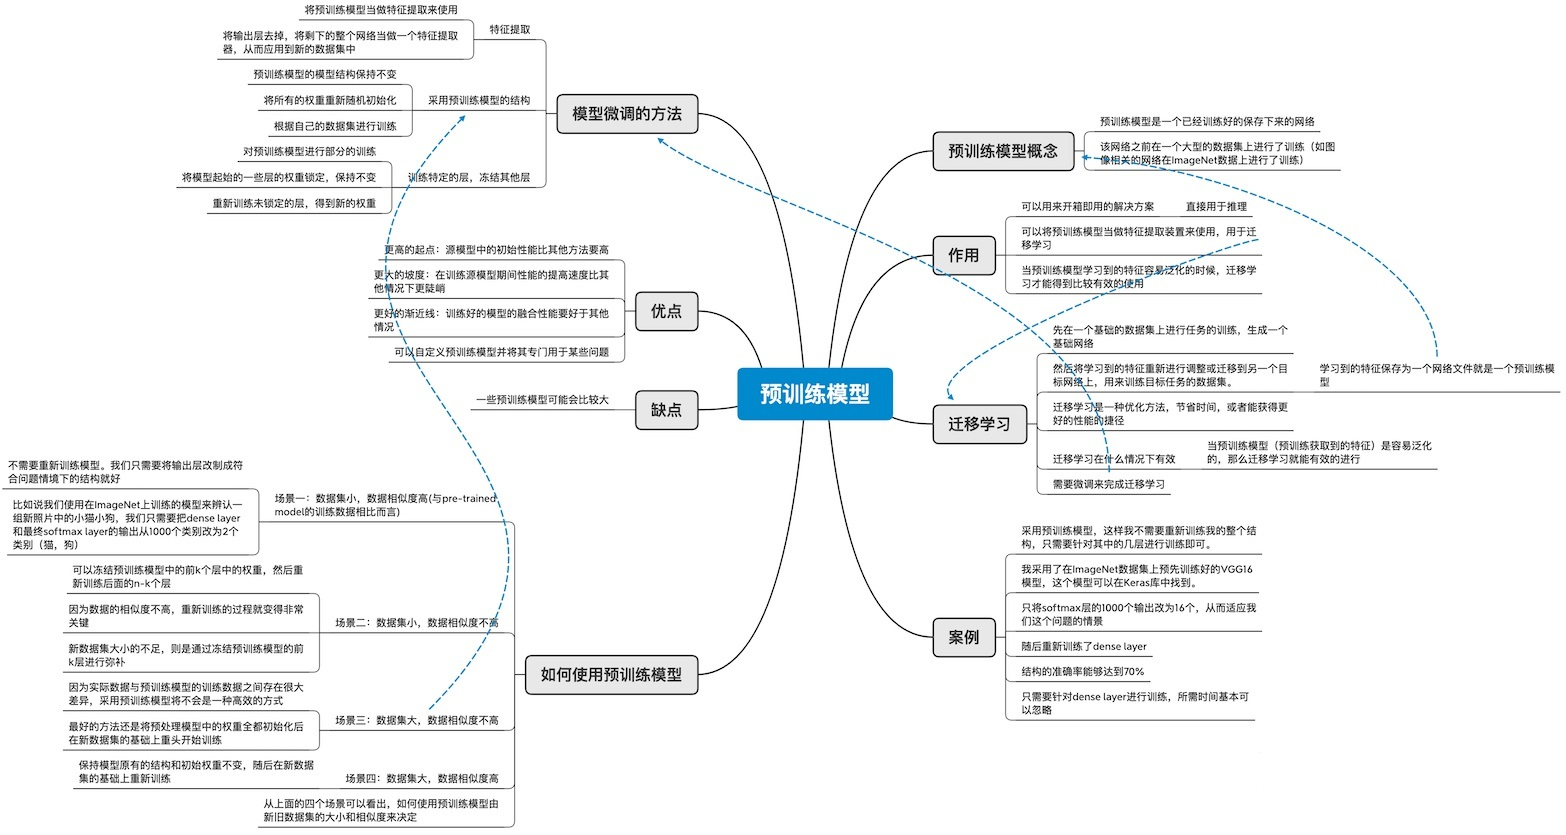
\includegraphics[width=\textwidth]{pics/pre-train.jpg}
	\caption{预训练模型(\href{https://www.zhihu.com/question/327642286/answer/1215812016}{出处})}
	\label{fig:pre-train}
\end{figure}
预训练通常在大量无监督的数据上学习(可以是无监督的学习任务、简单的有监督学习任务), 用无监督的数据帮助模型的参数收敛, 后续再在监督数据上进行调整. 




